\begin{slide}[toc=Hit-or-Miss method]{MC integration (Hit-or-Miss method)}
\null\vfill

  Lets do the following integration using MC method:
  
  $$\int_0^1 f(x)dx = \int_0^1 \left(\frac{1}{2}x\right) dx = \left.\frac{1}{2}\frac{x^2}{2}\right|_{0}^{1} = \frac{1}{4}$$

  \twocolumn
  {
    \sep
    \begin{itemize}
     \item take a random point from the $[0,1]\times[0,1]$ square
     \item compare it to your $f(x)$
     \item repeat $N$ times
     \item count $n$ points below the function
     \item you results is given by
     $$\int_0^1 f(x)dx = P_{\square} \cdot \frac{n}{N} = \frac{n}{N}$$
    \end{itemize}
  }
  {
    \usetikzlibrary{calc}

\begin{tikzpicture}

  \draw[>=latex, <->, thick] node[left, yshift = 4cm]{$y$} ++ (0, 4) -- (0, 0) -- node[below, xshift = 2cm]{$x$} ++ (4,0);
  
  \foreach \x in {1,...,200}
  {
    \pgfmathparse{rnd}
    \pgfmathsetmacro{\a}{2.9*\pgfmathresult + 0.05}
    \pgfmathparse{rnd}
    \pgfmathsetmacro{\b}{2.9*\pgfmathresult + 0.05}
    \pgfmathsetmacro{\c}{\a - 2.0 * \b}
        
    \ifthenelse{\lengthtest{\c pt > 0.2 pt}}{\draw[filled, color=pdcolor7] (\a, \b) circle (0.03);}{}
    \ifthenelse{\lengthtest{\c pt < - 0.2 pt}}{\draw[filled, color=pdcolor6] (\a, \b) circle (0.03);}{}
  }

  \draw[ultra thick] (0,0) -- node[yshift = 1.5cm, xshift = 2cm]{$f(x) = \frac{1}{2}x$} ++ (4,2);
  
  \draw[color=pdcolor3, dashed] node[left, yshift = 3cm]{1} ++ (0, 3) -- (3,3) -- node[yshift = -1.75cm]{1} (3, 0);
      
\end{tikzpicture}

  }
  
\vfill\null
\end{slide}

\begin{emptyslide}{MC integration results}
\null\vfill

  \twocolumn
  {
    
    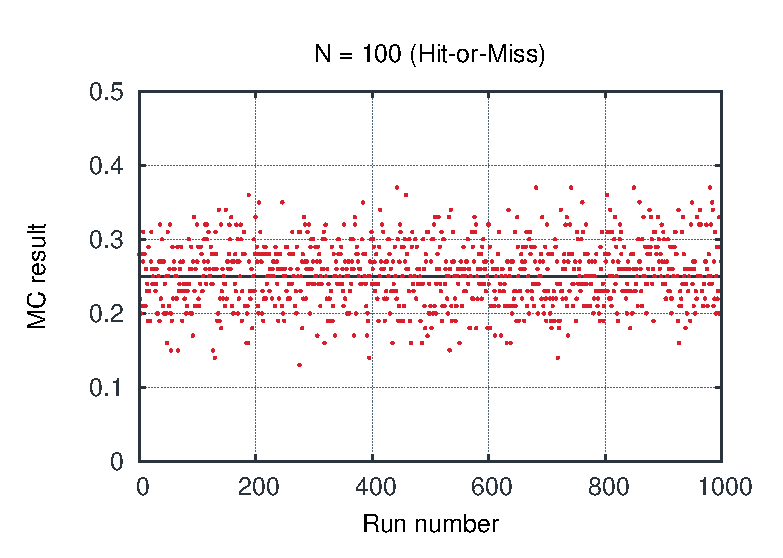
\includegraphics[width=\columnwidth]{figures/int100.eps}
    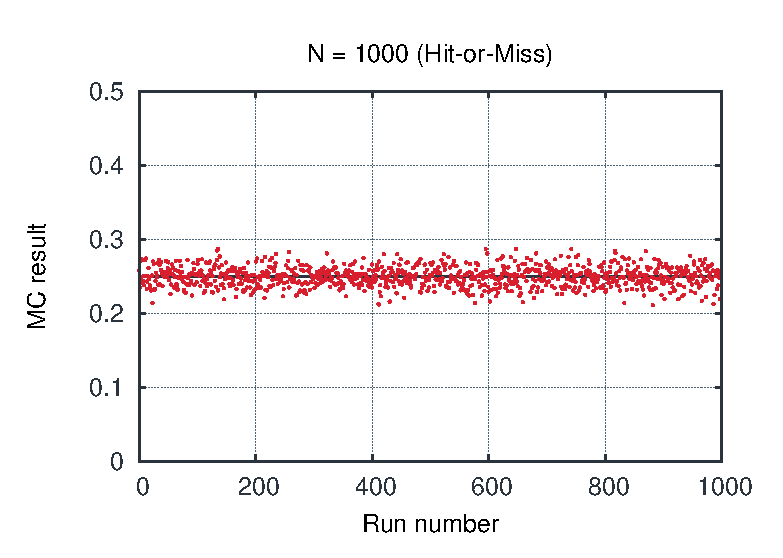
\includegraphics[width=\columnwidth]{figures/int1000.eps}
  }
  {
    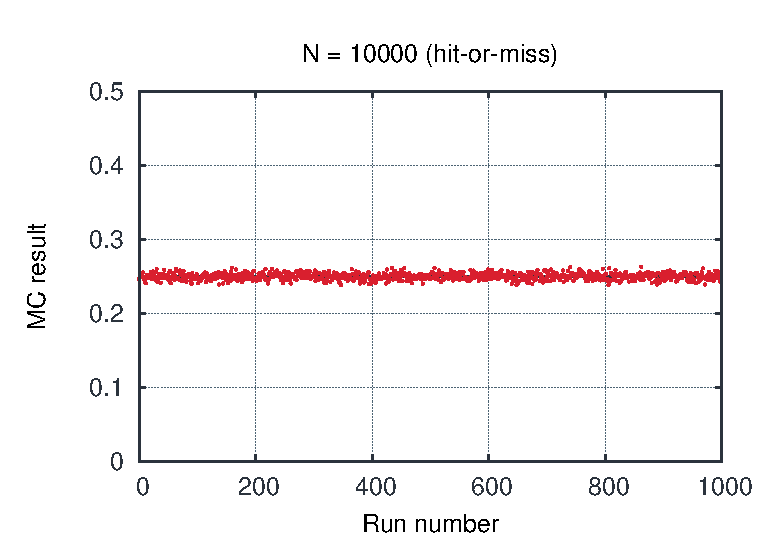
\includegraphics[width=\columnwidth]{figures/int10000.eps}
    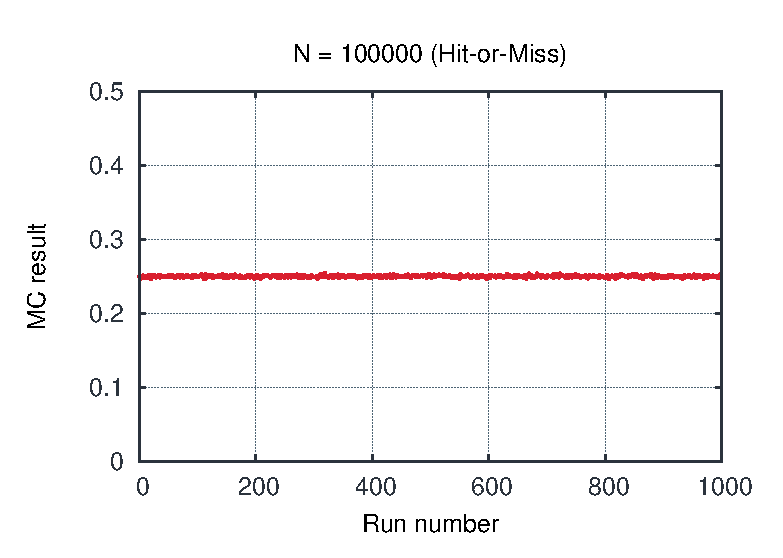
\includegraphics[width=\columnwidth]{figures/int100000.eps}
  }

\vfill\null
\end{emptyslide}


\begin{slide}{Optimization of MC}
\null\vfill

  \twocolumn
  {
    \scalebox{.75}{\usetikzlibrary{calc}

\begin{tikzpicture}

  \draw[>=latex, <->, thick] node[left, yshift = 4cm]{$y$} ++ (0, 4) -- (0, 0) -- node[below, xshift = 2cm]{$x$} ++ (4,0);
  
  \foreach \x in {1,...,200}
  {
    \pgfmathparse{rnd}
    \pgfmathsetmacro{\a}{2.9*\pgfmathresult + 0.05}
    \pgfmathparse{rnd}
    \pgfmathsetmacro{\b}{2.9*\pgfmathresult + 0.05}
    \pgfmathsetmacro{\c}{\a - 2.0 * \b}
        
    \ifthenelse{\lengthtest{\c pt > 0.2 pt}}{\draw[filled, color=pdcolor7] (\a, \b) circle (0.03);}{}
    \ifthenelse{\lengthtest{\c pt < - 0.2 pt}}{\draw[filled, color=pdcolor6] (\a, \b) circle (0.03);}{}
  }

  \draw[ultra thick] (0,0) -- node[yshift = 1.5cm, xshift = 2cm]{$f(x) = \frac{1}{2}x$} ++ (4,2);
  
  \draw[color=pdcolor3, dashed] node[left, yshift = 3cm]{1} ++ (0, 3) -- (3,3) -- node[yshift = -1.75cm]{1} (3, 0);
      
\end{tikzpicture}
}
  }
  {
    \scalebox{.75}{\usetikzlibrary{calc}

\begin{tikzpicture}

  \draw[>=latex, <->, thick] node[left, yshift = 4cm]{$y$} ++ (0, 4) -- (0, 0) -- node[below, xshift = 2cm]{$x$} ++ (4,0);
  
  \foreach \x in {1,...,200}
  {
    \pgfmathparse{rnd}
    \pgfmathsetmacro{\a}{2.9*\pgfmathresult + 0.05}
    \pgfmathparse{rnd}
    \pgfmathsetmacro{\b}{1.4*\pgfmathresult + 0.05}
    \pgfmathsetmacro{\c}{\a - 2.0 * \b}
        
    \ifthenelse{\lengthtest{\c pt > 0.2 pt}}{\draw[filled, color=pdcolor7] (\a, \b) circle (0.03);}{}
    \ifthenelse{\lengthtest{\c pt < - 0.2 pt}}{\draw[filled, color=pdcolor6] (\a, \b) circle (0.03);}{}
  }

  \draw[ultra thick] (0,0) -- node[yshift = 1.5cm, xshift = 2cm]{$f(x) = \frac{1}{2}x$} ++ (4,2);
  
  \draw[color=pdcolor3, dashed] node[left, yshift = 1.5cm]{0.5} ++ (0, 1.5) -- (3,1.5) -- node[yshift = -1.75cm]{1} (3, 0);
      
\end{tikzpicture}
}
  }

  \begin{itemize}
   \item You want to avoid drawing ``red'' points as they do not contribute to your integral
   \item You can choose any rectangle as far as it contains maximum of $f(x)$ in given range
  \end{itemize}

\vfill\null
\end{slide}

\begin{slide}[toc=]{Optimization of MC}
\null\vfill

  \twocolumn
  {
    \begin{itemize}
      \item Lets consider the following function:
  
      $$F(Q^2) = \frac{1}{(1 + Q^2)^2}$$
      {\it\color{pdcolor3} more or less dipole form factor}
      
      \item Integrating this function over $Q^2$ is highly inefficient
      
      \item However, one can integrate by substitution to get better performance, e.g.
      
      $$x = \mbox{log}_{10}(Q^2)$$
      
    \sep{\it\color{pdcolor6}don't forget about Jacobian}

    \end{itemize}

  }
  {
    \usetikzlibrary{calc}

\pgfplotsset{every  tick/.style={pdcolor3,}, minor x tick num=1,}

\begin{tikzpicture}

  \begin{axis}[xlabel = $Q^2$, ylabel = $F(Q^2)$, ylabel near ticks, domain=1:10, scale=0.5, axis lines = left, inner axis line style={>=latex}, ymin = 0, ymax = 0.275, xmin = 1, xmax = 10.5]
    
    \addplot[mark=none, color=pdcolor1, ultra thick] {1 / (1 + x) / (1 + x)};
    \addplot[mark=none, dashed, color=pdcolor3, thick] coordinates {(1,0.25) (10,0.25) (10,0)};

    
    \foreach \x in {1,...,200}
    {
      \pgfmathparse{rnd}
      \pgfmathsetmacro{\a}{9.0*\pgfmathresult + 0.95}
      \pgfmathparse{rnd}
      \pgfmathsetmacro{\b}{0.23*\pgfmathresult + 0.01}
      \pgfmathsetmacro{\c}{\b - 1 / (1 + \a) / (1 + \a)}
      	  
      \ifthenelse{\lengthtest{\c pt > 0.01 pt}}{\addplot[mark=*, mark size = 1pt, color=pdcolor6] coordinates {(\a, \b)};}{}
      \ifthenelse{\lengthtest{\c pt < -0.01 pt}}{\addplot[mark=*, mark size = 1pt, color=pdcolor7] coordinates {(\a, \b)};}{}
    }
    
  \end{axis}

\end{tikzpicture}
    \vspace{-10pt}
    \usetikzlibrary{calc}

\pgfplotsset{every  tick/.style={pdcolor3,}, minor x tick num=1,}

\begin{tikzpicture}

  \begin{axis}[xlabel = {$x = \mbox{log}_{10}(Q^2)$}, ylabel = $F(x)$, ylabel near ticks, domain=-2:1, scale=0.5, axis lines = left, inner axis line style={>=latex}, ymin = 0, ymax = 1.25, xmin = -2, xmax = 1.25]
    
    \addplot[mark=none, color=pdcolor1, ultra thick] {1 / (1 + 10^x) / (1 + 10^x)};
    \addplot[mark=none, dashed, color=pdcolor3, thick] coordinates {(-2,1) (1,1) (1,0)};
    
    \foreach \x in {1,...,200}
    {
      \pgfmathparse{rnd}
      \pgfmathsetmacro{\a}{-2.90*\pgfmathresult + 0.95}
      \pgfmathparse{rnd}
      \pgfmathsetmacro{\b}{0.90*\pgfmathresult + 0.05}
      \pgfmathsetmacro{\d}{-0.175 * (\a + 2) * (\a + 2) + 1}
      \pgfmathsetmacro{\c}{\b - \d}
      	  
      \ifthenelse{\lengthtest{\c pt > 0.1 pt}}{\addplot[mark=*, mark size = 1pt, color=pdcolor6] coordinates {(\a, \b)};}{}
      \ifthenelse{\lengthtest{\c pt < - 0.1 pt}}{\addplot[mark=*, mark size = 1pt, color=pdcolor7] coordinates {(\a, \b)};}{}
    }
    
  \end{axis}

\end{tikzpicture}
    
  }
    
\vfill\null
\end{slide}

\begin{slide}[toc=Crude method]{MC integration (Crude method)}
\null\vfill

  Lets do the following integration using MC method once again:
  
  $$\int_0^1 f(x)dx = \int_0^1 \left(\frac{1}{2}x\right) dx = \left.\frac{1}{2}\frac{x^2}{2}\right|_{0}^{1} = \frac{1}{4}$$
  \twocolumn
  {
    \begin{itemize}
      \item One can approximate integral
      \vspace{-5pt}
      $$\int_a^b f(x) dx \approx \frac{b - a}{N}\sum_{i=1}^{N} f(x_i)$$
     
      where $x_i$ is a random number from $[a, b]$
      
      \item It can be shown that Crude method is more accurate than Hit-or-Miss
      
      \item We will skip the math and look at some comparisons
      
    \end{itemize}
  }
  {
    \usetikzlibrary{calc}

\begin{tikzpicture}

  \draw[>=latex, <->, thick] node[left, yshift = 4cm]{$y$} ++ (0, 4) -- (0, 0) -- node[below, xshift = 2cm]{$x$} ++ (4,0);
  
  \foreach \x in {1,...,14}
  {
    \pgfmathparse{rnd}

    \pgfmathsetmacro{\a}{0.2 * \x + 0.05 + 0.1 * \pgfmathresult - 0.05}
        
    \draw[filled, color=pdcolor7] (\a, 0) circle (0.03);
    
    \draw[thin, color=pdcolor3, dashed] (\a, 0) -- (\a, 0.5*\a);
  }

  \draw[ultra thick] (0,0) -- node[yshift = 1.5cm, xshift = 2cm]{$f(x) = \frac{1}{2}x$} ++ (4,2);
        
\end{tikzpicture}

  }

\vfill\null
\end{slide}

\begin{emptyslide}{Methods comparison}
\null\vfill

  \twocolumn
  {
    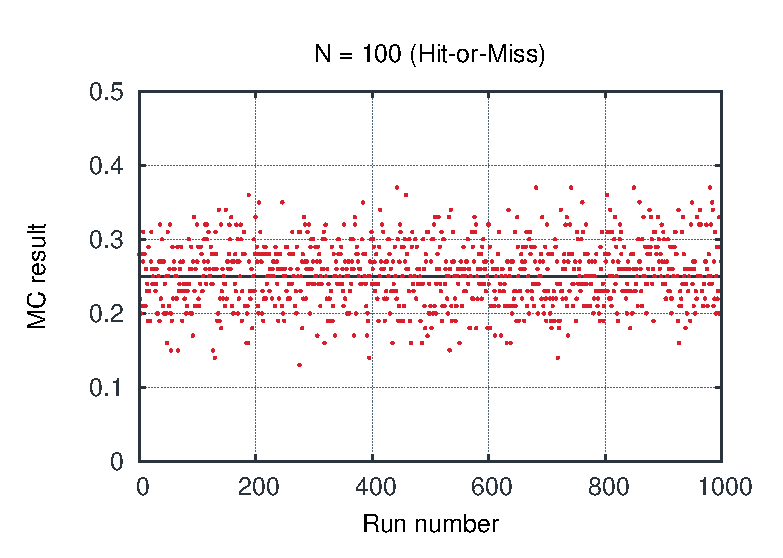
\includegraphics[width=\columnwidth]{figures/int100.eps}
    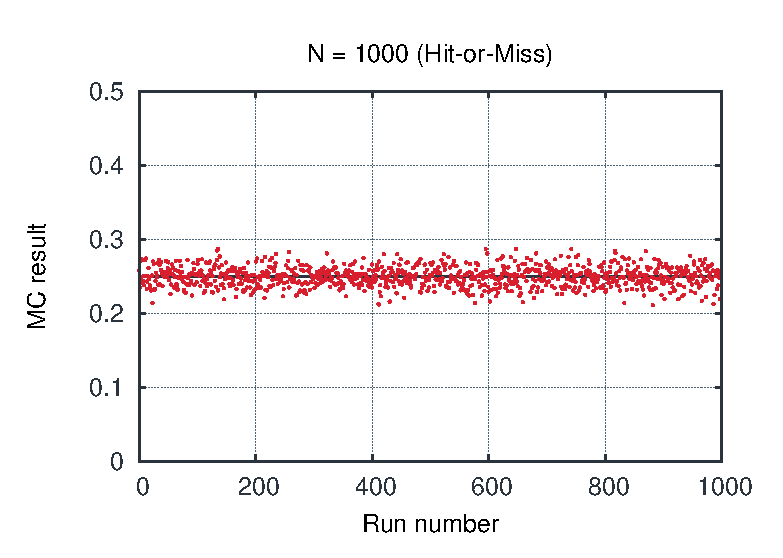
\includegraphics[width=\columnwidth]{figures/int1000.eps}
  }
  {
    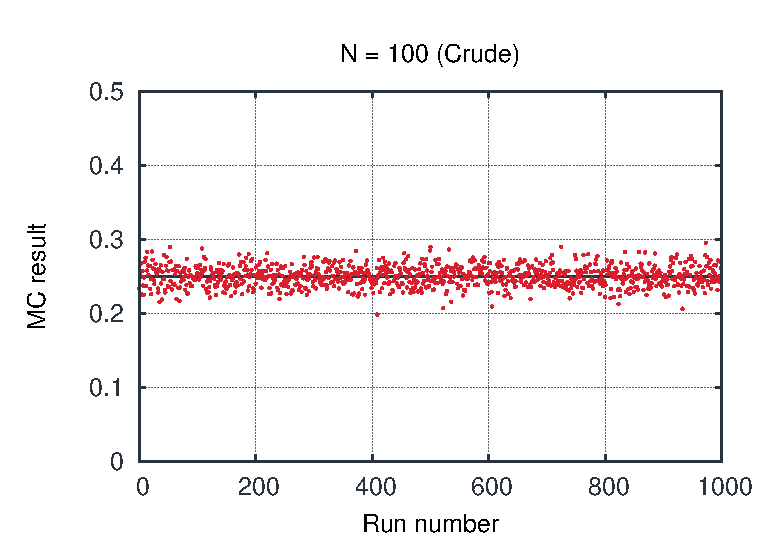
\includegraphics[width=\columnwidth]{figures/int2100.eps}
    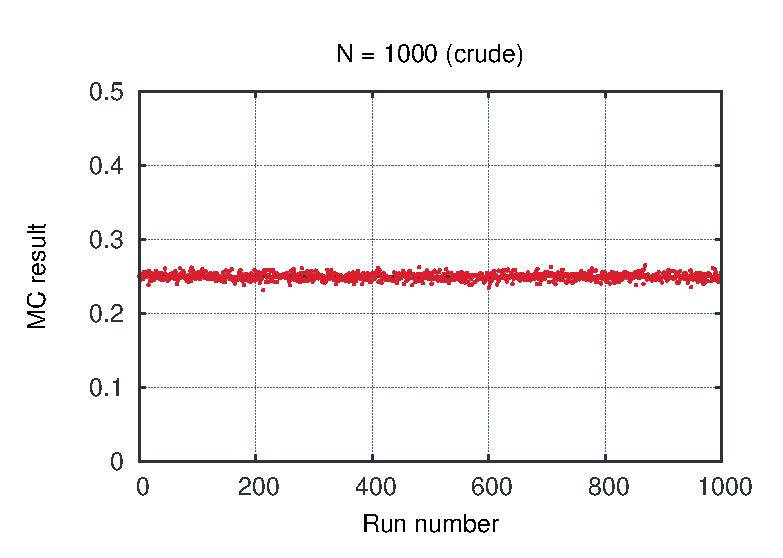
\includegraphics[width=\columnwidth]{figures/int21000.eps}
  }

\vfill\null
\end{emptyslide}